
\subsection*{task 1.4 [20 points] \\[1ex] finding maximally different images}

So far, you only had to do what the problem specifications asked you to do. In this task, you need to get creative!

Reread matrix $\mat{X}$ from task 1.1 into memory but \emph{do not normalize it to zero mean}. Now, think of / invent an algorithm that selects $k>2$ out of the $n$ columns of $\mat{X}$ such that the selected data vectors are as far apart as possible. 

Mathematically, the problem considered in this task is a subset selection problem and we can formalize it as follows: given $X = \{ \vec{x}_1, \ldots, \vec{x}_n \}$, solve
\begin{align*}
S^* = \amax{S \subset X} & \sum_{\vec{x}_i \in S} \sum_{\vec{x}_j \in S} \dsq{\vec{x}_i}{\vec{x}_j} \\
\st \; & \; \; \lvert S \rvert = k
\end{align*}
\textbf{NOTE:} this problem is actually way more difficult than it may appear at first sight; in fact, it is NP-complete and an \textit{efficient} algorithm that is \textit{guaranteed} to find the optimal $S^*$ for very large sets $X$ and arbitrary choices of $k$ remains elusive to this date. \vspace{1ex}

%%%%%
%%%%%
%%%%% enter your code into the following environment
%%%%%
%%%%%
\begin{python}
# past your code here


\end{python}
%%%%%
%%%%%
%%%%%
%%%%%
%%%%%
\vspace{2cm}

Test your algorithm for several choices of $k$, say $k \in \{ 25, 50, 100 \}$, and visualize the extracted columns in terms of tiny images. For instance, for $k \in \{ 4, 9, 16 \}$, your result could look like this:
%%%%%
%%%%%
%%%%% enter your plots here, i.e. replace "t1-4-k*.png" by the names of the graphics files you created
%%%%%
%%%%%
\begin{center}
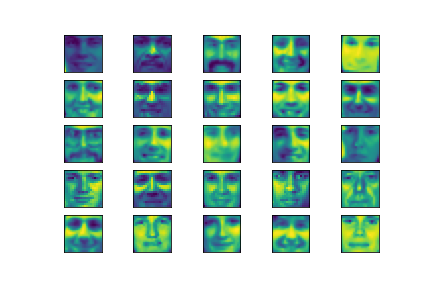
\includegraphics[width=0.25\textwidth]{t1-4-k4.png} 
\quad
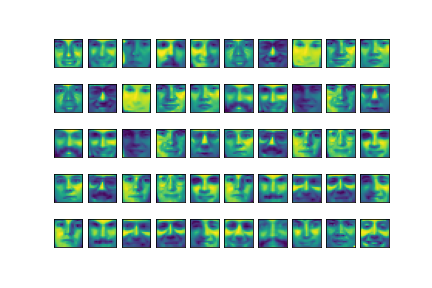
\includegraphics[width=0.25\textwidth]{t1-4-k9.png}
\quad
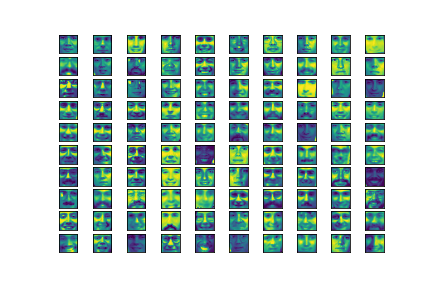
\includegraphics[width=0.25\textwidth]{t1-4-k16.png}
\end{center}
%%%%%
%%%%%
%%%%%
%%%%%
%%%%%
Simply replace the above three images with your results for $k \in \{25, 50, 100\}$.






